\documentclass[11pt,conference]{IEEEtran}
\usepackage[margin=1in]{geometry}
\usepackage[T1]{fontenc}
\usepackage{amsmath}
\usepackage{graphicx}
\usepackage{booktabs}
\usepackage{array}
\usepackage{url}
\usepackage[nocompress]{cite}
\usepackage{tikz}
\usetikzlibrary{arrows.meta,positioning,fit,calc}

\begin{document}

\title{CS 550/ECE 552 Final Report:\\Replicating the Hawkeye and Mockingjay
Cache Replacement Policies in gem5}

\author{\IEEEauthorblockN{Vito Wang, Endong Dai, and Xiaotian Tong}
\IEEEauthorblockA{Duke University}}

\maketitle

\begin{abstract}
Hawkeye and Mockingjay are last-level cache (LLC) replacement policies that
learn from Belady's optimal algorithm. Hawkeye learns whether the optimal
policy would keep the lines that each instruction brings in, and Mockingjay
learns how far in the future these lines will be reused. Both were proposed
and evaluated in trace-driven simulators, and gem5 includes neither of them. We
implement both policies in gem5 and fix three gem5 problems that would
otherwise corrupt their training. Python reference models replay gem5's logs
and agree with every prediction, priority, and eviction on three
microbenchmarks and two SPEC CPU2017 benchmarks. On six SPEC CPU2017
benchmarks with 1 to 4\,MB LLCs, Mockingjay removes 11.6\% and 19.2\% of the
LLC misses of mcf at 2 and 4\,MB, close to twice the reductions of Hawkeye,
and improves IPC by up to 14.4\%. This ordering agrees with the original
papers. Both policies lose to LRU on omnetpp. Using LLC traces, we show that
LRU is within 1\% of the optimal policy on this benchmark, and that 65\% of
Hawkeye's extra misses come from instructions whose PCs never access the sets
that Hawkeye samples, so their predictions are never corrected. We also find
that our gem5 version of Mockingjay, which cannot bypass the LLC, has at most
4.7\% more misses than the original design would.
\end{abstract}

%% ------------------------------------------------------------------
\section{Introduction}

The last-level cache (LLC) is the last on-chip structure before DRAM. An LLC
miss needs a DRAM access that takes hundreds of cycles, and an out-of-order
processor can hide only part of this latency. When the LLC is full, the
replacement policy chooses which line to evict, and this choice largely decides
the miss rate. The common least-recently-used (LRU) policy fails when a program
cycles through a working set larger than the cache, and when data that is never
reused pushes useful lines out. Improved policies handle some of these
patterns, for example by inserting new lines with a low priority~\cite{rrip} or
by learning which instructions bring in lines that are reused~\cite{ship}.
However, each is built around a particular class of access patterns.

Belady's algorithm~\cite{belady}, also called OPT, evicts the line whose next
use lies furthest in the future. It is optimal but needs future knowledge.
Hawkeye~\cite{hawkeye} computes what OPT would have done on past accesses and
learns which instructions bring in lines that OPT would keep. On
memory-intensive SPEC CPU2006 benchmarks, it improves IPC over LRU by 8.4\%.
Its follow-up, Mockingjay~\cite{mockingjay}, predicts how far in the future
each line will be reused, which lets it order lines the way OPT does. On a
single core without prefetching, it improves IPC over LRU by 5.7\%, compared
with 4.4\% for Hawkeye. Both policies were evaluated in trace-driven
simulators built for the Cache Replacement Championships~\cite{crc2}, and
gem5~\cite{gem5,gem5v20} includes neither of them.

Moving these policies into gem5 is not a direct translation. gem5's caches
pass more kinds of requests to the policy, such as writebacks, clean-eviction
notices, and instruction fetches, and the policy cannot refuse an insertion.
Each of these differences can change what the policies learn. This project
replicates both policies in gem5 and asks whether their reported behavior holds
in this setting. We make the following contributions.

\begin{itemize}
\item We implement Hawkeye and Mockingjay in gem5, together with variants that
always keep instruction lines, and we fix three gem5 problems that would
otherwise corrupt their training (Section~\ref{sec:impl}).
\item We validate both implementations against reference models, event by
event (Section~\ref{sec:valid}).
\item We compare both policies with five built-in gem5 policies on
microbenchmarks and on six SPEC CPU2017 benchmarks with three LLC sizes
(Section~\ref{sec:perf}).
\item We use LLC traces to explain the results, i.e., how much room OPT leaves
on each benchmark, why both policies lose on omnetpp, why Mockingjay loses on
xalancbmk with a 4\,MB LLC, and what the lack of bypassing costs
(Section~\ref{sec:analysis}).
\end{itemize}

%% ------------------------------------------------------------------
\section{Background and Related Work}

\emph{Heuristic policies.} LRU and LFU rank lines by recency or
frequency~\cite{hp6}. DIP~\cite{dip} inserts most lines at the LRU position and
uses set dueling, i.e., a few sets that each run a fixed policy, to choose the
better insertion policy at run time. RRIP~\cite{rrip} predicts how soon each
line will be re-referenced with a 2- or 3-bit counter per line. SRRIP inserts
lines with a long predicted interval, BRRIP inserts most lines with a distant
one, and DRRIP chooses between the two through set dueling. A previous CS 550
project evaluated these policies in gem5, and we use them as baselines. They
treat every incoming line alike, so they cannot tell a reused array from a
stream that runs at the same time.

\emph{Reuse prediction.} SDBP~\cite{sdbp} uses a small sampler to learn, for
each program counter (PC), whether a line is dead after that PC accesses it.
SHiP~\cite{ship} learns for each PC signature whether its lines receive hits. Perceptron-based predictors combine the PC with other features such as
address bits~\cite{perceptron}. These predictors learn from the behavior of a
heuristic policy, e.g., whether a line hit under LRU, so they inherit its
limits.

\emph{Learning from Belady's algorithm.} Hawkeye~\cite{hawkeye} instead learns
from OPT's decisions on past accesses, and its authors released a version of
it for the 2nd Cache Replacement Championship (CRC2)~\cite{crc2}. Harmony~\cite{harmony} extends it to systems
with prefetchers by learning from a variant of OPT that favors demand hits.
Glider~\cite{glider} adds the recent history of PCs to Hawkeye's predictor.
Mockingjay~\cite{mockingjay} replaces Hawkeye's binary prediction with a
prediction of the reuse distance, and it evicts the line that it expects to be
reused furthest in the future.

\emph{Our work.} The policies above were evaluated in trace-driven simulators
with simple models of the core and the memory system. We replicate the two
policies at the center of this line of work in gem5, where the LLC sees the
full traffic of a cycle-level system. Our focus is on validating the two
implementations and on explaining where the policies lose, rather than on a
new policy.

%% ------------------------------------------------------------------
\section{The Two Policies}
\label{sec:policies}

\begin{figure*}[t]
\centering
\resizebox{\textwidth}{!}{%
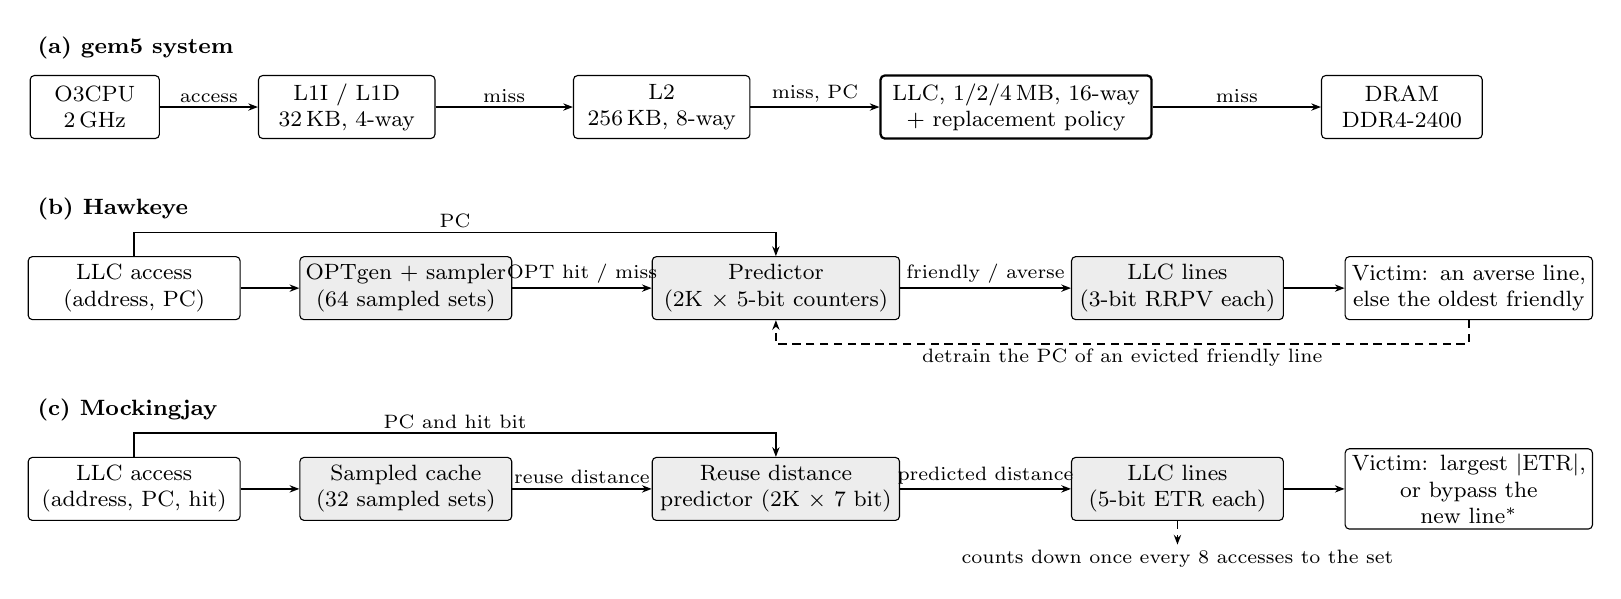
\begin{tikzpicture}[font=\footnotesize,
  box/.style={draw, rounded corners=1.5pt, align=center, inner sep=2pt,
              minimum height=0.8cm, text width=2.55cm},
  st/.style={box, fill=black!7},
  arr/.style={-{Stealth[length=3.5pt]}, semithick},
  lab/.style={font=\scriptsize, inner sep=1.5pt},
  row/.style={font=\footnotesize\bfseries, anchor=west}]
\def\ca{1.3}\def\cb{4.75}\def\cc{9.45}\def\cd{14.55}\def\ce{18.25}
% (a) the gem5 system
\node[row] at (-0.05,0.75) {(a) gem5 system};
\node[box, text width=1.5cm] (cpu) at (0.8,0) {O3CPU\\2\,GHz};
\node[box, text width=2.1cm] (l1) at (4.0,0) {L1I / L1D\\32\,KB, 4-way};
\node[box, text width=2.1cm] (l2) at (8.0,0) {L2\\256\,KB, 8-way};
\node[box, text width=3.3cm, thick] (llc) at (12.5,0)
  {LLC, 1/2/4\,MB, 16-way\\+ replacement policy};
\node[box, text width=1.9cm] (dram) at (17.4,0) {DRAM\\DDR4-2400};
\draw[arr] (cpu) -- node[lab, above] {access} (l1);
\draw[arr] (l1) -- node[lab, above] {miss} (l2);
\draw[arr] (l2) -- node[lab, above] {miss, PC} (llc);
\draw[arr] (llc) -- node[lab, above] {miss} (dram);
% (b) Hawkeye
\begin{scope}[yshift=-2.3cm]
\node[row] at (-0.05,1.0) {(b) Hawkeye};
\node[box] (ha) at (\ca,0) {LLC access\\(address, PC)};
\node[st] (og) at (\cb,0) {OPTgen + sampler\\(64 sampled sets)};
\node[st, text width=3.0cm] (hp) at (\cc,0) {Predictor\\(2K $\times$ 5-bit counters)};
\node[st] (rr) at (\cd,0) {LLC lines\\(3-bit RRPV each)};
\node[box, text width=3.0cm] (hv) at (\ce,0) {Victim: an averse line,\\else the oldest friendly};
\draw[arr] (ha) -- (og);
\draw[arr] (og) -- node[lab, above] {OPT hit / miss} (hp);
\draw[arr] (hp) -- node[lab, above] {friendly / averse} (rr);
\draw[arr] (rr) -- (hv);
\draw[arr] (ha.north) -- ++(0,0.3) -| node[lab, pos=0.25, above] {PC} (hp.north);
\draw[arr, densely dashed] (hv.south) -- ++(0,-0.3) -| node[lab, pos=0.25, below]
  {detrain the PC of an evicted friendly line} (hp.south);
\end{scope}
% (c) Mockingjay
\begin{scope}[yshift=-4.85cm]
\node[row] at (-0.05,1.0) {(c) Mockingjay};
\node[box] (ma) at (\ca,0) {LLC access\\(address, PC, hit)};
\node[st] (sc) at (\cb,0) {Sampled cache\\(32 sampled sets)};
\node[st, text width=3.0cm] (rdp) at (\cc,0) {Reuse distance\\predictor (2K $\times$ 7 bit)};
\node[st] (etr) at (\cd,0) {LLC lines\\(5-bit ETR each)};
\node[box, text width=3.0cm] (mv) at (\ce,0) {Victim: largest $|$ETR$|$,\\or bypass the new line$^{\ast}$};
\draw[arr] (ma) -- (sc);
\draw[arr] (sc) -- node[lab, above] {reuse distance} (rdp);
\draw[arr] (rdp) -- node[lab, above] {predicted distance} (etr);
\draw[arr] (etr) -- (mv);
\draw[arr] (ma.north) -- ++(0,0.3) -| node[lab, pos=0.25, above] {PC and hit bit} (rdp.north);
\draw[arr, densely dashed] (etr.south) -- ++(0,-0.3) node[lab, below]
  {counts down once every 8 accesses to the set};
\end{scope}
\end{tikzpicture}}
\caption{(a) The gem5 system. Demand requests carry their PC to the LLC.
Writebacks and the L2's clean-eviction notices carry none, and the policies
handle them separately. (b) Hawkeye and (c) Mockingjay. Shaded boxes are the
structures that each policy adds, with sizes for a 2\,MB LLC. $^{\ast}$gem5
cannot bypass, so our version inserts the line as the next victim
(Section~\ref{sec:impl}).}
\label{fig:arch}
\end{figure*}

\subsection{Hawkeye}

Fig.~\ref{fig:arch}(b) shows Hawkeye. \textbf{OPTgen} reconstructs OPT's
decisions on a sample of 64 sets. When a line is accessed again, OPTgen checks
whether OPT could have kept the line since its previous access without
exceeding the cache capacity at any point in between. A \textbf{sampler}
remembers the PC that last accessed each line of these sets. The
\textbf{predictor} keeps a 5-bit counter for each hashed PC. It counts up when
OPT would have hit and down when OPT would have missed. A line whose PC counter
is in the upper half is \emph{cache-friendly} and is inserted with a 3-bit
re-reference prediction value (RRPV) of 0. Otherwise it is
\emph{cache-averse} and is inserted with RRPV 7. Hawkeye evicts an averse line
first. If there is none, it evicts the oldest friendly line and, if the line is
in a sampled set, lowers the counter of the PC that brought it in.

Where the paper and the authors' CRC2 code differ, we follow the code. For
example, the code uses 2K 5-bit counters instead of 8K 3-bit counters, and it
limits OPTgen to 14 lines of a 16-way set.

\subsection{Mockingjay}

Fig.~\ref{fig:arch}(c) shows Mockingjay. The \textbf{sampled cache} records
recent accesses to 32 sampled sets. When a line is accessed again, it measures
the reuse distance, i.e., the number of accesses to the set since the previous
access. A line that is not reused within 127 accesses is treated as never
reused. The \textbf{reuse distance predictor (RDP)} learns the typical reuse
distance of the lines brought in by each signature, i.e., a hash of the PC and
of whether the access hit. Each LLC line keeps a 5-bit \textbf{estimated time
remaining (ETR)}. It starts at the predicted reuse distance divided by 8 and
counts down once every 8 accesses to the set, so it becomes negative when the
line is overdue. Mockingjay evicts the line with the largest $|$ETR$|$, which is
either reused furthest in the future or most overdue. If the incoming line
would be reused later than every line in the set, Mockingjay does not insert
it. We follow a public ChampSim implementation, whose parameters match the
paper.

\emph{Storage.} For a 2\,MB LLC, the added structures of our Hawkeye take
30.0\,KB (28\,KB in the paper, because the CRC2 code records every access in
OPTgen), and those of Mockingjay take 31.91\,KB, the same as the paper.

%% ------------------------------------------------------------------
\section{Implementation in gem5}
\label{sec:impl}

A gem5 replacement policy keeps state for each line and implements four calls.
\texttt{reset} is called when a line is filled, \texttt{touch} when it hits,
\texttt{invalidate} when it is removed, and \texttt{getVictim} receives the
lines of one set and returns the victim. The policy sees a whole set only in
\texttt{getVictim}, and it cannot decline an insertion. Each policy is a new
class of about 650 lines of C++ with a debug flag and statistics, and an
install script adds it to an unmodified gem5 v23.0.0.1.

\emph{Hawkeye.} When Hawkeye inserts a friendly line, it ages the other lines in
the set, but \texttt{reset} receives only the new line. gem5 always calls
\texttt{getVictim} on the same set right before the fill, so Hawkeye remembers
that set and ages it in \texttt{reset}. A statistic counts fills whose set does
not match, and it stayed zero in every run. Writebacks from the L2 carry no PC.
As in the CRC2 code, Hawkeye does not train on them, and a line filled by a
writeback is inserted as cache-averse.

\emph{Mockingjay.} gem5 cannot bypass a fill. However, a line that Mockingjay
would bypass gets an ETR larger than every other line in the set, so inserting
it normally makes it the next victim. This is an approximation, because the new
line still evicts one line, and Section~\ref{sec:bypass} measures its cost.
Also, the policy cannot age a whole set every 8 accesses. Each line instead
records the set's aging count when its ETR is set, and the current ETR is
computed when the line is compared. As in the ChampSim code, a line filled by a writeback gets
ETR $-15$, which makes it the first candidate for eviction.

\emph{gem5 problems.} While validating Hawkeye, we found and fixed three gem5
problems. First, the L2 notifies the LLC of every clean eviction, and gem5
passes these notifications to the policy as if they were accesses. Hawkeye
trained on 8.7 million of them in mcf, so both policies now ignore them.
Second, gem5 dropped the PC when the L1 forwarded a software prefetch, so 28\%
of omnetpp's LLC accesses had no PC. We now copy the PC to the forwarded
request. Third, gem5's x86-64 \texttt{newfstatat} system call used the wrong
file-status structure, so omnetpp and gcc failed to start. After these fixes,
the only LLC requests without a PC are the L2's writebacks and clean-eviction
notices.

\emph{Instruction lines.} In gem5, the PC of an instruction fetch is the fetch
address itself. Each instruction line thus has its own PC, and its prediction
is trained only if the line itself falls in a sampled set. We therefore also test two
variants that are not in the papers. HawkeyeI always inserts instruction lines
as friendly. MockingjayI inserts them with ETR 0 and keeps them out of the
sampled cache.

%% ------------------------------------------------------------------
\section{Methodology}
\label{sec:method}

\emph{System.} We use gem5 in syscall-emulation mode with the x86 out-of-order
CPU model (O3CPU) and the cache hierarchy of Fig.~\ref{fig:arch}(a), which
follows Table~2 of the Hawkeye paper. The LLC is mostly inclusive, and there is
no hardware prefetcher. The baselines are gem5's LRU, SRRIP, BRRIP, DRRIP, and
SHiP. DRRIP uses 32 dueling sets for each of its two policies.

\emph{Workloads.} We use the speed versions of mcf, omnetpp, and xalancbmk from
SPEC CPU2017~\cite{spec17}, and the rate versions of gcc, xz, and deepsjeng,
because the speed versions of these three need 7 to 15\,GB of memory and our
instance has 15\,GB. An atomic CPU skips the first one billion instructions,
and the caches and the policy are still accessed during this step. The O3CPU
then runs 50 million instructions of warmup and 200 million measured
instructions, the same lengths as in the Hawkeye paper. We report demand LLC
misses per kilo-instruction (MPKI), the fraction of LRU's misses that each
policy removes, and the IPC speedup over LRU. All six benchmarks use a 2\,MB
LLC. For mcf, xalancbmk, and omnetpp, where the policies differ most, we also
use 1\,MB and 4\,MB.

\emph{Microbenchmarks.} \emph{fit} loops over a 1\,MB array, so it fits in the
LLC. \emph{thrash} loops over a 3\,MB array, so each set cycles through 24 lines
with 16 ways. \emph{mix} alternates a pass over a 1\,MB reused array with a
24\,MB stream that is never reused. Each program prints a checksum, which must
be the same under every policy.

\emph{Validation.} The debug flag of each policy logs every LLC event and every
decision. A Python reference model reads only the order of events and the way
that gem5 chose from the log. It computes everything else on its own and
compares each decision with gem5's.

\emph{Offline trace analysis.} To explain the results, we log every LLC event
of a SPEC run from the end of the fast-forward and replay it through Python
models of LRU, Belady's OPT, and Mockingjay with and without bypassing. This is
fair because the LLC demand stream hardly depends on the LLC policy, i.e., the
number of LLC accesses differs by less than 0.3\% across policies. The models
start with an empty cache at the end of the fast-forward, while gem5's caches
and predictors are already warm. From the start of a program, the Mockingjay
model and gem5 agree on every access. After the fast-forward, their miss counts
differ by $-5.2\%$ to $+2.8\%$ (except on xalancbmk at 4\,MB, where the
model's cache never fills), so we compare policies only within the models.

%% ------------------------------------------------------------------
\section{Functional Validation}
\label{sec:valid}

\begin{table}[t]
\centering
\caption{Event-by-event check of gem5 against the reference models. The
microbenchmarks run 6 passes, and the SPEC runs execute 30 million
instructions from the start. ``Victims'' counts evictions of valid lines.}
\label{tab:valid}
\setlength{\tabcolsep}{2.5pt}
\begin{tabular}{@{}llrrr@{}}
\toprule
Policy & Program & Accesses & Victims & Mismatch \\
\midrule
Hawkeye & fit & 115,691 & 0 & 0 \\
& thrash & 345,069 & 254,872 & 0 \\
& mix & 902,156 & 1,513,747 & 0 \\
& gcc & 99,081 & 33,291 & 0 \\
& omnetpp & 40,268 & 59 & 0 \\
\midrule
Mockingjay & fit, thrash, mix & 1,362,923 & 1,571,344 & 0 \\
& gcc & 98,908 & 29,939 & 0 \\
& omnetpp & 40,268 & 59 & 0 \\
\bottomrule
\end{tabular}
\end{table}

Table~\ref{tab:valid} summarizes the check. For Hawkeye, the model compares
every OPTgen decision, predictor counter, prediction, RRPV, and victim,
including the aging of other lines and the detraining of evicted friendly
lines. For Mockingjay, it compares every ETR and victim. Victims include those
caused by writebacks, and there is no mismatch in any run.
Because gem5's victims depend on all earlier decisions, a single wrong counter
or priority would soon show up as a wrong victim. The omnetpp run rarely
fills its cache, so victim choices are covered mainly by the other runs.

A check that never fails could also be too weak, so we introduced two errors
into the Hawkeye model and replayed the thrash log. Breaking ties among
friendly lines in favor of the first way instead of the last caused 101 victim
mismatches. Removing the detraining caused 32,760 counter mismatches and 34,717
RRPV mismatches. We also replayed the Mockingjay logs through a version of the
model that chooses its own victims instead of following gem5, and it hit and
missed on exactly the same gcc and omnetpp accesses as gem5. Finally, we reran
the Mockingjay experiments on a second machine, and every miss count and IPC
was identical.

\begin{table}[t]
\centering
\caption{LLC miss rate (\%) on the microbenchmarks. fit has only compulsory
misses under every policy (15.0\% with 6 passes, 5.0\% with 20). OPT comes from
a model of the access stream without writebacks.}
\label{tab:micro}
\setlength{\tabcolsep}{4.5pt}
\begin{tabular}{@{}lrrrr@{}}
\toprule
& \multicolumn{2}{c}{thrash} & \multicolumn{2}{c}{mix} \\
\cmidrule(lr){2-3}\cmidrule(l){4-5}
Policy & 6 passes & 20 passes & 6 passes & 20 passes \\
\midrule
LRU, SRRIP & 100 & 100 & 100 & 100 \\
BRRIP & \textbf{46.8} & \textbf{40.6} & 96.4 & 95.4 \\
DRRIP & 61.7 & 56.1 & 99.1 & 98.8 \\
SHiP & 90.0 & 80.0 & 100 & 100 \\
Hawkeye & 48.1 & 41.0 & \textbf{88.3} & \textbf{88.7} \\
Mockingjay & 58.3 & 44.5 & 96.5 & 91.2 \\
\midrule
OPT (model) & 42.9 & 36.5 & 87.3 & 88.4 \\
\bottomrule
\end{tabular}
\end{table}

Table~\ref{tab:micro} shows the microbenchmarks. All policies behave as their
designs predict, and every checksum is identical across policies. In thrash, LRU and SRRIP miss on
every access because they always evict the line that is needed next. BRRIP and
Hawkeye keep part of the array, and with 20 passes they come within 4.5 points
of OPT. In mix, Hawkeye separates the reused array from the stream and stays
within 1 point of OPT. Mockingjay learns more slowly, because it decides that a
line is never reused only after 127 accesses to its set, and in our model it
starts to keep the reused array only in the fourth pass. Its gap to Hawkeye shrinks from 10.2 to 3.4 points on thrash and
from 8.2 to 2.5 points on mix between 6 and 20 passes. The variants HawkeyeI
and MockingjayI give the same results as Hawkeye and Mockingjay here, because
few instruction lines reach the LLC.

%% ------------------------------------------------------------------
\section{Performance on SPEC CPU2017}
\label{sec:perf}

\begin{figure*}[t]
\centering
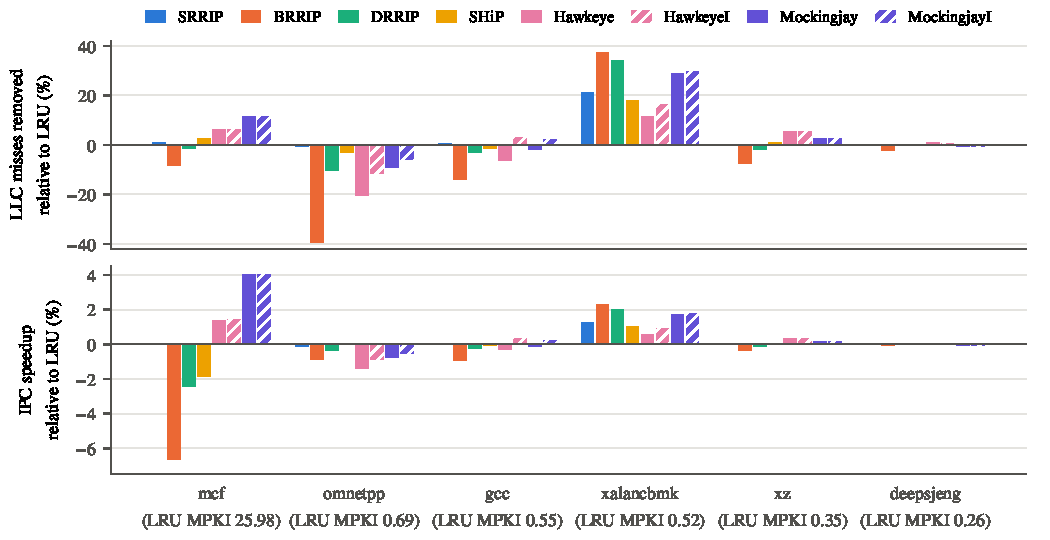
\includegraphics[width=\textwidth]{fig/spec_2mb.pdf}
\caption{LLC misses removed and IPC speedup relative to LRU with a 2\,MB LLC. A
negative value means more misses or a lower IPC than LRU. Benchmarks are sorted
by their LRU MPKI. The hatched bars are the variants that always keep
instruction lines.}
\label{fig:spec}
\end{figure*}

\begin{table*}[t]
\centering
\caption{LLC misses removed (\%) / IPC speedup (\%) relative to LRU for three
LLC sizes. ``Best baseline'' is the built-in policy (SRRIP, BRRIP, DRRIP, or
SHiP) with the highest IPC.}
\label{tab:sweep}
\setlength{\tabcolsep}{5pt}
\begin{tabular}{@{}llrlllll@{}}
\toprule
& LLC & LRU MPKI & Best baseline & Hawkeye & HawkeyeI & Mockingjay & MockingjayI \\
\midrule
mcf & 1\,MB & 32.08 & SHiP $+$7.8 / $+$1.2 & $+$6.3 / $+$1.6 & $+$6.3 / $+$1.6 & $+$8.3 / $+$1.0 & $+$8.3 / $+$1.0 \\
 & 2\,MB & 25.98 & SRRIP $+$1.0 / 0.0 & $+$6.3 / $+$1.4 & $+$6.3 / $+$1.4 & $+$11.6 / $+$4.0 & $+$11.6 / $+$4.0 \\
 & 4\,MB & 22.27 & SRRIP $+$2.7 / $+$1.5 & $+$10.8 / $+$7.6 & $+$10.8 / $+$7.6 & \textbf{$+$19.2 / $+$14.4} & \textbf{$+$19.2 / $+$14.4} \\
\midrule
xalancbmk & 1\,MB & 4.74 & BRRIP \textbf{$+$52.8 / $+$21.3} & $+$19.5 / $+$6.1 & $+$22.6 / $+$7.5 & $+$45.6 / $+$17.2 & $+$46.6 / $+$18.0 \\
 & 2\,MB & 0.52 & BRRIP $+$37.4 / $+$2.3 & $+$11.5 / $+$0.6 & $+$16.5 / $+$0.9 & $+$28.7 / $+$1.7 & $+$29.6 / $+$1.8 \\
 & 4\,MB & 0.15 & DRRIP $+$2.2 / 0.0 & $+$1.3 / 0.0 & $+$4.5 / $+$0.1 & $-$30.0 / $-$0.5 & $-$29.8 / $-$0.5 \\
\midrule
omnetpp & 1\,MB & 0.96 & SHiP $-$15.5 / 0.0 & $-$12.8 / $-$1.2 & $-$4.1 / $-$0.5 & $-$17.3 / $-$1.4 & $-$8.1 / $-$0.6 \\
 & 2\,MB & 0.69 & SHiP $-$3.0 / 0.0 & $-$20.4 / $-$1.4 & $-$11.6 / $-$0.9 & $-$9.2 / $-$0.8 & $-$5.7 / $-$0.6 \\
 & 4\,MB & 0.68 & SHiP $-$0.2 / $-$0.3 & $-$9.9 / $-$1.1 & $-$5.6 / $-$0.9 & $-$1.8 / $-$1.0 & $-$1.7 / $-$1.0 \\
\bottomrule
\end{tabular}
\end{table*}

Fig.~\ref{fig:spec} compares all policies with a 2\,MB LLC, and
Table~\ref{tab:sweep} adds the 1\,MB and 4\,MB LLCs for the three benchmarks
where the policies differ most.

\emph{mcf.} mcf has 38 times the MPKI of any other benchmark at 2\,MB. It is
also the only one with an MPKI above 1, the criterion that the Mockingjay paper
uses to select memory-sensitive applications. Here both policies clearly beat every built-in policy,
and Mockingjay beats Hawkeye. At 2\,MB, Mockingjay removes 11.6\% of the misses
and improves IPC by 4.0\%, while Hawkeye removes 6.3\% and improves IPC by
1.4\%. No built-in policy improves IPC by more than 0.1\%. The advantage of both
policies grows with the LLC, and at 4\,MB Mockingjay removes 19.2\% of the
misses and improves IPC by 14.4\%. The ordering of Mockingjay, Hawkeye, and
SHiP matches both papers.

\emph{xalancbmk.} The working set of xalancbmk lies between 1 and 4\,MB.
Mockingjay removes far more misses than Hawkeye at 1 and 2\,MB, e.g., 28.7\%
against 11.5\% at 2\,MB, and most of the difference comes from data lines. However, BRRIP removes even more (37.4\%). At 4\,MB, Mockingjay has 30\%
more misses than LRU, but the MPKI rises only from 0.15 to 0.20 and IPC drops
by 0.5\%. Section~\ref{sec:xalanc} explains this loss.

\emph{omnetpp, gcc, xz, and deepsjeng.} On these benchmarks, no policy changes
IPC by more than 1.5\%. On omnetpp, every policy has more misses than LRU at
every size. At 2\,MB, BRRIP and Hawkeye lose the most (39.2\% and 20.4\%). On gcc, Hawkeye loses
6.2\% while HawkeyeI gains 3.1\%. Section~\ref{sec:analysis} shows why there is
little to gain on these benchmarks and why the original policies lose.

\emph{Comparison with the papers.} Our gains are smaller than the reported
ones, i.e., 8.4\% for Hawkeye on memory-intensive SPEC CPU2006 and 5.7\% for
Mockingjay on applications with an MPKI above 1. We see three reasons. First,
both papers average over memory-intensive benchmarks, while five of our six
benchmarks have an MPKI below 1 with a 2\,MB LLC and leave OPT little room
(Section~\ref{sec:room}). Second, our measured region follows a fixed
fast-forward instead of a SimPoint, and on omnetpp it falls in the program's
setup phase (Section~\ref{sec:omnetpp}). Third, gem5 sends instruction fetches
and writebacks through the same LLC, and both affect what the policies learn.
On mcf, the one benchmark that meets the Mockingjay paper's criterion, the
papers' ordering holds.

%% ------------------------------------------------------------------
\section{Analysis}
\label{sec:analysis}

\subsection{How much room does OPT leave?}
\label{sec:room}

Replaying the LLC traces through LRU and OPT from the same empty cache shows
how many misses any policy could remove. OPT has 27--29\% fewer misses than LRU
on mcf at all three sizes and 55\% fewer on xalancbmk at 2\,MB. On the other
benchmarks, the gap is small, i.e., 4.8\% on xz, 2.8\% on gcc, 0.9\% on
omnetpp, and 0.2\% on deepsjeng. On omnetpp, 136,232 of the 136,233 misses of
OPT are first accesses to a line since the fast-forward, so the misses come
from new data rather than from evictions. A policy that deviates from LRU on
these benchmarks therefore has much more to lose than to gain, which explains
why even SHiP and DRRIP lose on omnetpp.

\subsection{Instruction lines}

Because each instruction line has its own PC (Section~\ref{sec:impl}), most
instruction lines are never trained, and those that are trained can be
predicted wrongly. On omnetpp at 2\,MB, Hawkeye predicts
13\% of the instruction fetches as cache-averse although OPT keeps them, and
its LLC instruction misses rise from 662 under LRU to 11,113. Mockingjay
suffers less, with 4,271 instruction misses. HawkeyeI brings instruction misses
to the level of LRU or below on every benchmark, and MockingjayI does nearly
the same. As a result, gcc turns from a 6.2\% loss into a 3.1\% gain for
Hawkeye, and the loss on omnetpp drops from 20.4\% to 11.6\%. These results
suggest that a PC-based policy needs separate handling for instruction lines.

\subsection{omnetpp: untrained PCs}
\label{sec:omnetpp}

\begin{table}[t]
\centering
\caption{Hawkeye's misses on omnetpp (2\,MB) that LRU does not have, by what
Hawkeye last did with the line.}
\label{tab:omnetpp}
\setlength{\tabcolsep}{4pt}
\begin{tabular}{@{}lrr@{}}
\toprule
& Data & Instr. \\
\midrule
Hawkeye misses, LRU hits & 17,899 & 10,525 \\
\quad Predicted averse, OPT keeps & 15,374 & 10,521 \\
\qquad PC never in a sampled set & 8,405 & 9,989 \\
\quad Filled by a writeback & 2,505 & 3 \\
LRU misses, Hawkeye hits & 316 & 123 \\
\bottomrule
\end{tabular}
\end{table}

To find the remaining loss on omnetpp, we traced Hawkeye at 2\,MB and looked at
every access that misses under Hawkeye but hits under LRU
(Table~\ref{tab:omnetpp}). Most of these lines were predicted cache-averse at
their previous access although OPT would have kept them, and most were reused
within 16 accesses to their set. Among the
lines predicted averse, 55\% of the data lines and 95\% of the instruction
lines had been brought in by a PC that never touched one of the 64 sampled
sets during the trace, so Hawkeye never trained on it. For example, \texttt{PatternMatcher::matches} accesses
only 24 lines in the trace, about 130 times each, and none of them lies in a
sampled set. Its counter stays at 3 throughout, below the threshold of 16, so
each access is predicted averse, while OPT keeps 99\% of them. Sampling 64 of
2048 sets works well for PCs that touch many lines, but a PC that touches a few
hot lines may never be sampled.

The other two causes are smaller. PCs in shared library code such as
\texttt{memcpy} and \texttt{malloc} bring in lines with mixed reuse, which a
per-PC prediction cannot separate. Also, 14\% of the lost data lines had been
evicted from the LLC while the L2 still held them, and the L2's later writeback
inserted them as cache-averse. LRU instead places a writeback at the most
recently used position. Mockingjay loses for a similar reason. 90\% of its
extra misses at 2\,MB are lines that it had evicted as never reused (ETR 15),
yet 82\% of the lost lines were used again within 16 accesses to their set.

The trace also shows that our measured region of omnetpp is not
representative of the whole program. Most LLC accesses come from
\texttt{memcpy}, \texttt{malloc}, the traversal of the network description, and
\texttt{PatternMatcher}, which suggests that omnetpp is still building its
simulation network after one billion instructions.

\subsection{xalancbmk: reuse beyond Mockingjay's horizon}
\label{sec:xalanc}

At 4\,MB, Mockingjay has 6,833 misses on xalancbmk that LRU does not have. Using
gem5's own eviction log, we found that 83\% of these lines were evicted with
ETR $-15$, i.e., as far overdue as the ETR can express, and that 87\% of them had
not been used for at least 128 accesses to their set. Mockingjay tracks reuse
distances only up to 127 accesses to a set. Beyond this horizon, every
overdue line has ETR $-15$, and lines with the same $|$ETR$|$ are chosen by
their position in the set rather than by their age. LRU still evicts the
oldest line. During the trace, xalancbmk touches only 4\% more lines than a
4\,MB LLC holds, so LRU keeps almost every line that will be used again, even
after a long gap. With a 2\,MB LLC, LRU also misses most reuses that long, so
they do not count against Mockingjay. Only 43\% of the lines that Mockingjay
loses at 2\,MB lie beyond the horizon, and it removes 28.7\% of LRU's misses.
The horizon of 8 times the associativity therefore limits Mockingjay when the
LLC is large enough to keep lines across longer reuses.

\subsection{The cost of not bypassing}
\label{sec:bypass}

\begin{table}[t]
\centering
\caption{Mockingjay with and without bypassing in the offline model, and the
estimated effect on gem5's results, i.e., the misses removed relative to
LRU by gem5's version and by the original design with bypassing.}
\label{tab:bypass}
\setlength{\tabcolsep}{3pt}
\begin{tabular}{@{}llrrrr@{}}
\toprule
& & Bypassed & Misses & \multicolumn{2}{c}{Misses removed} \\
\cmidrule(l){5-6}
& LLC & fills & saved & gem5 & bypass \\
\midrule
mcf & 1\,MB & 68\% & 1.2\% & 8.3\% & 9.4\% \\
& 2\,MB & 82\% & 0.9\% & 11.6\% & 12.4\% \\
& 4\,MB & 99\% & 4.7\% & 19.2\% & 23.0\% \\
xalancbmk & 2\,MB & 39\% & 1.9\% & 28.7\% & 30.1\% \\
omnetpp & 2\,MB & 3\% & $-$1.1\% & $-$9.2\% & $-$10.3\% \\
\bottomrule
\end{tabular}
\end{table}

Table~\ref{tab:bypass} replays each Mockingjay trace through the model with
and without bypassing. ``Bypassed fills'' is the fraction of the misses that the
original design does not insert, and ``misses saved'' is the reduction in
misses from bypassing them. We scale gem5's miss count by this reduction to
estimate the original design in gem5. Bypassing helps clearly only on mcf with
a 4\,MB LLC, where it would raise the misses removed from 19.2\% to about
23\%. Elsewhere the difference is at most 1.9\%, and it is below 0.1\% on gcc,
xz, and deepsjeng. On omnetpp, bypassing even adds misses, because a wrongly
bypassed line gets no chance to hit. The cost is small even when most fills
would be bypassed, because such a line is inserted as the next victim and is
usually evicted by the next fill to the set, so these lines rarely displace
useful ones. Our approximation thus does not change any ranking.

%% ------------------------------------------------------------------
\section{Conclusion}

We implemented Hawkeye and Mockingjay in gem5 and validated both against
reference models on every decision. Along the way, we found that gem5 passes
clean-eviction notices to replacement policies, drops the PC of forwarded
software prefetches, and gives each instruction line its own PC, and that each
of these affects the training of a PC-based policy. With these issues
handled, the main result of the papers holds on the memory-intensive mcf. With
2 and 4\,MB LLCs, Mockingjay removes close to twice as many misses as Hawkeye,
and both beat every built-in policy. On benchmarks with a low MPKI, LRU is
already close to OPT, so the policies gain little and can lose, as on omnetpp. Our traces point to two limits of the
designs. Sampling a few sets leaves some hot PCs untrained, and Mockingjay
cannot rank lines whose reuse lies beyond 8 times the associativity. Lifting
these limits and adding prefetchers and multiple cores are natural next steps.

%% ------------------------------------------------------------------
\section*{Division of Labor}

\textbf{Vito Wang} implemented Hawkeye and its variants in gem5, found and fixed
the clean-eviction and software-prefetch problems, wrote the Hawkeye reference
model, validated both policies event by event, ran the offline trace analyses,
and analyzed the SPEC CPU2017 results. \textbf{Endong Dai} set up the gem5
system with the O3CPU, the LLC, and the fast-forward step, fixed the
\texttt{newfstatat} problem, built the SPEC CPU2017 benchmarks, wrote the
microbenchmarks, ran the baselines, implemented Mockingjay in gem5, and
collected and plotted the statistics. \textbf{Xiaotian Tong} wrote the
Mockingjay reference model, estimated the storage of both policies, computed
the expected microbenchmark results, and mapped Mockingjay onto gem5's
interface. All three wrote this report.

%% ------------------------------------------------------------------
\begin{thebibliography}{99}

\bibitem{rrip}
A. Jaleel, K. B. Theobald, S. C. Steely Jr., and J. Emer, ``High performance
cache replacement using re-reference interval prediction (RRIP),'' in
\emph{Proc. ISCA}, 2010.

\bibitem{ship}
C.-J. Wu, A. Jaleel, W. Hasenplaugh, M. Martonosi, S. C. Steely Jr., and
J. Emer, ``SHiP: Signature-based hit predictor for high performance caching,''
in \emph{Proc. MICRO}, 2011.

\bibitem{belady}
L. A. Belady, ``A study of replacement algorithms for a virtual-storage
computer,'' \emph{IBM Systems Journal}, vol. 5, no. 2, pp. 78--101, 1966.

\bibitem{hawkeye}
A. Jain and C. Lin, ``Back to the future: Leveraging Belady's algorithm for
improved cache replacement,'' in \emph{Proc. ISCA}, 2016.

\bibitem{mockingjay}
I. Shah, A. Jain, and C. Lin, ``Effective mimicry of Belady's MIN policy,'' in
\emph{Proc. HPCA}, 2022.

\bibitem{crc2}
The 2nd Cache Replacement Championship (CRC2), held with ISCA 2017.

\bibitem{gem5}
N. Binkert \emph{et al.}, ``The gem5 simulator,'' \emph{ACM SIGARCH Comput.
Archit. News}, vol. 39, no. 2, pp. 1--7, 2011.

\bibitem{gem5v20}
J. Lowe-Power \emph{et al.}, ``The gem5 simulator: Version 20.0+,''
arXiv:2007.03152, 2020.

\bibitem{hp6}
J. L. Hennessy and D. A. Patterson, \emph{Computer Architecture: A Quantitative
Approach}, 6th ed. Morgan Kaufmann, 2019.

\bibitem{dip}
M. K. Qureshi, A. Jaleel, Y. N. Patt, S. C. Steely Jr., and J. Emer, ``Adaptive
insertion policies for high performance caching,'' in \emph{Proc. ISCA}, 2007.

\bibitem{sdbp}
S. M. Khan, Y. Tian, and D. A. Jim\'enez, ``Sampling dead block prediction for
last-level caches,'' in \emph{Proc. MICRO}, 2010.

\bibitem{perceptron}
E. Teran, Z. Wang, and D. A. Jim\'enez, ``Perceptron learning for reuse
prediction,'' in \emph{Proc. MICRO}, 2016.

\bibitem{harmony}
A. Jain and C. Lin, ``Rethinking Belady's algorithm to accommodate
prefetching,'' in \emph{Proc. ISCA}, 2018.

\bibitem{glider}
Z. Shi, X. Huang, A. Jain, and C. Lin, ``Applying deep learning to the cache
replacement problem,'' in \emph{Proc. MICRO}, 2019.

\bibitem{spec17}
Standard Performance Evaluation Corporation, ``SPEC CPU2017,''
\url{https://www.spec.org/cpu2017/}.

\end{thebibliography}

\end{document}
